\documentclass[11pt]{article}
\usepackage[letterpaper,margin=1in]{geometry}
\usepackage{amsmath,amssymb}
\usepackage{lmodern}
\usepackage[T1]{fontenc}
\usepackage{graphicx}
\usepackage{booktabs}
\usepackage{tabularx}
\usepackage{array}
\usepackage{enumitem}
\usepackage[hidelinks]{hyperref}
\usepackage{microtype}
\setlength{\parindent}{0pt}
\setlength{\parskip}{6pt}
\emergencystretch=2em
\setlist{itemsep=2pt,topsep=2pt}
\newcommand{\code}[1]{\texttt{#1}}
\newcommand{\Q}{\mathcal{Q}}

\title{How EXCALI works: from the paper to the solver}
\author{Matthew Staber}
\date{October 24, 2026}

\begin{document}
\maketitle

\section{Overview}

EXCALI (EXact Cauchy-Analytic Lambert Integration) solves Lambert's problem with the contour-integral idea of Negrete and Abdelkhalik, shrunk to a rectangle of zero height so that it needs only real arithmetic. Given two positions, a time of flight and a revolution count, it returns both endpoint velocities for elliptic, parabolic, hyperbolic and multi-revolution transfers.

The root of the time equation is never iterated toward. A closed-form starter places an interval around it. One 8-node quadrature then reads the root off as a ratio of two sums. A 3-node quadrature runs only when the first one's own error estimate is above rounding. When the starter misses (0 to 0.8\% of solves), further rectangles run inside a shrinking bracket. No Newton step is taken anywhere in the root solve.

On the mixed benchmark of \href{https://github.com/Ossama-Abdelkhalik-Lab/Lamberts-Comparison}{Lamberts-Comparison}, EXCALI takes 0.91 times ivLam's time overall on Apple silicon and 1.18 times on a Linux x86-64 runner. Its maximum errors are lower than ivLam's in 8 of the 10 feasible classes, and both are at rounding level in the other two.

The chain of versions is:
\begin{enumerate}
  \item \textbf{The paper} (Negrete and Abdelkhalik, JGCD 2025): the root as a ratio of two contour integrals over a circle, using the trapezoidal rule.
  \item \textbf{Exact v1}: the paper's circles in code, a coarse circle and then a fine one, with complex trigonometry.
  \item \textbf{Exact v2.2}: one thin rectangle around a guess from a lookup table, plus one Newton step. Zero-revolution ellipses only.
  \item \textbf{EXCALI}: the zero-height limit of that rectangle, staged, with closed-form starters and coverage of every conic and revolution count.
\end{enumerate}
The Exact originals are preserved unchanged in the EXCALI repository as \code{original/}.

\section{The starting point: the paper}

The paper is A.~Negrete and O.~O.~Abdelkhalik, ``Exact Solution to Lambert's Problem Using Contour Integrals,'' \emph{Journal of Guidance, Control, and Dynamics} 48(4), 2025 (\href{https://doi.org/10.2514/1.G008499}{doi:10.2514/1.G008499}; not redistributed here). It turns root finding into pole finding.

\paragraph{Time equation.} The paper uses the universal-variable form of Bate, Mueller and White. With Stumpff functions $C(z)$ and $S(z)$, the geometric constant $A$ and $y(z) = r_1 + r_2 + A\,(zS-1)/\sqrt{C}$, the time of flight is
\begin{equation}
  \sqrt{\mu}\,\Delta t(z) = \chi(z)^3 S(z) + A\sqrt{y(z)}, \qquad \chi = \sqrt{y/C}.
\end{equation}
Here $z = \Delta E^2$ for an ellipse and $z<0$ for a hyperbola. Zero-revolution ellipses have $0<z<4\pi^2$, and $m$ revolutions lie in $4m^2\pi^2 \le z < 4(m+1)^2\pi^2$.

\paragraph{Root as a pole.} The paper defines $f(z) = 1/\big(\chi^3 S + A\sqrt{y} - \sqrt{\mu}\,\Delta t\big)$. The wanted root $z^*$ is a simple pole of $f$. Cauchy's theorem applied to $(z-z^*)f(z)$ on any closed contour $C$ around that pole alone gives
\begin{equation}
  z^* = \frac{\oint_C z\,f(z)\,dz}{\oint_C f(z)\,dz}.
\end{equation}
The formula is exact; only the two integrals are approximated.

\paragraph{Quadrature and contours.} The integrals are taken on circles with the composite trapezoidal rule. It converges exponentially there because $f$ is analytic near the circle. The paper uses three families of circles:
\begin{itemize}
  \item \textbf{Zero-revolution ellipse:} centred at $2\pi^2$ with radius $2\pi^2-\varepsilon$, which covers the whole elliptic interval.
  \item \textbf{Hyperbola:} a lower bound $z_l$ from a reversed power series of $\Delta t$ about the parabola, then a circle on $[z_l,0]$.
  \item \textbf{$m$ revolutions:} one circle over the whole band, where two poles share the contour. Four moments $I_k = \oint z^k f\,dz$ give a quadratic whose two roots are the two branches. Complex roots mean the time is below the minimum, so no transfer exists.
\end{itemize}
The velocities then follow from the Lagrange coefficients $f$, $g$ and $\dot g$.

The paper's examples use a large circle followed by a second circle of radius 2 around its estimate. With $N=6$ points the second circle reaches a mean relative error of $8.8\times10^{-13}$ in $z$.

\paragraph{What the paper leaves open.} It gives no rule that guarantees a contour holds exactly one pole, apart from the zero-revolution ellipse. It covers neither near-parabolic cancellation nor transfers near $180^\circ$. It also does not avoid complex trigonometry at every node, which dominates the cost.

\section{From the paper to EXCALI}

Each step keeps the paper's exact ratio and changes how its two integrals are taken. The steps below are in the order they were made.

\subsection*{Step 1: Exact v1, circles in code}
Exact v1 implemented the paper directly. It used a coarse half circle (centre $2\pi^2$, radius 19.5, 17 points), then a fine half circle of radius at most 2 (9 points) and one complex-step Newton correction. Conjugate symmetry, $f(\bar z) = \overline{f(z)}$, means only the upper half is needed. Every fine node still needed a complex $\sin$, $\cos$, $\sinh$ and $\cosh$, so it took about 900\,ns per problem. The coarse circle also missed roots near 0 and $4\pi^2$, so 0.1\% of its answers had errors above 0.17.

\subsection*{Step 2: Exact v2.2, a thin rectangle}
Exact v2.2 replaced the circles with one thin rectangle $[a,b]\times[-\varepsilon,\varepsilon]$ around a guess, with height $\varepsilon = 10^{-7}$. Only the upper half is evaluated: 8 Gauss--Legendre nodes on the top edge and one midpoint on each side. Taking the moment about the centre $c$ keeps small root increments from being lost:
\begin{equation}
  z^* = c + \frac{\operatorname{Im}\sum_k W_k\,(z_k-c)\,f(z_k)}{\operatorname{Im}\sum_k W_k\,f(z_k)}.
\end{equation}
The nodes sit a fixed distance from the real axis. Exact v2.2 therefore stored every node-dependent factor for 125 precomputed rectangles, and took the guess from a $64\times32$ lookup table. One Newton step followed. It reached 99\,ns per problem with errors comparable to ivLam, but only for zero-revolution ellipses. It was supplied in two builds of the same algorithm: \code{exact\_ser.F90}, a scalar kernel with a sine table compiled without vectorization, and \code{exact\_vect.F90}, a branch-free kernel with a polynomial sine that processes blocks of 32 problems with SIMD instructions. Both are kept byte for byte in \code{original/}.

\subsection*{Step 3: the zero-height limit}
This is the step that defines EXCALI. Expand each node of v2.2's discrete rectangle in its height $\varepsilon$, using $f(x+i\varepsilon) = f(x) + i\varepsilon f'(x) + O(\varepsilon^2)$ for real $f$ on the real axis:
\begin{itemize}
  \item \textbf{Top edge, $b$ to $a$:} Gauss--Legendre with half-width $L$ gives an imaginary part of $-\varepsilon L\sum_i w_i f'(x_i)$.
  \item \textbf{Right side, $b$ to $b+i\varepsilon$:} $f(b)$ times $i\varepsilon$, imaginary part $\varepsilon f(b)$.
  \item \textbf{Left side, $a+i\varepsilon$ to $a$:} imaginary part $-\varepsilon f(a)$.
\end{itemize}
The imaginary parts sum to $\varepsilon\,\Q[f'] + O(\varepsilon^3)$, where
\begin{equation}
  \Q[g'] = g(c+L) - g(c-L) - L\sum_i w_i\,g'(x_i).
\end{equation}
$\Q$ is the quadrature error of an exact derivative. It vanishes for any polynomial the rule integrates exactly and is nonzero only because of the pole. The factor $\varepsilon$ cancels in the ratio, so the limit $\varepsilon\to0$ is
\begin{equation}
  \boxed{\;z^* = c + \frac{\Q\big[((x-c)f)'\big]}{\Q\big[f'\big]}, \qquad f = \frac{1}{T(x)-t}.\;}
\end{equation}

\paragraph{Why it is still exact for one pole.} Write $f = R/(x-p) + h(x)$ with $h$ analytic. Then
\[
  (x-c)\,f = R + \frac{R\,(p-c)}{x-p} + (x-c)\,h,
\]
and the constant $R$ drops out of $\Q$. The pole parts give the ratio $p-c$ exactly, for any $p$ inside the interval and any node count. Only the analytic remainder $h$ limits accuracy. Gauss--Legendre quadrature of $h'$ converges like $(L/2R)^{2n}$, where $R$ is the distance from $c$ to the nearest other singularity of $f$.

The limit removes the complex arithmetic. Each node needs $T$ and $T'$ at a real point, and $T'$ has a closed form. The rectangle no longer has to be precomputed, so it can be centred anywhere and sized to the problem.

\subsection*{Step 4: real coordinates instead of $z$}
EXCALI works in the half anomaly $v = \sqrt{z}/2$ (so $z = 4v^2$) for ellipses and $w = \sqrt{-z}/2$ for hyperbolas. In $v$, with the larger radius normalized to 1 and $\mu=1$:
\begin{equation}
  y(v) = y_0 + 2b\sin^2(v/2), \qquad T(v) = \sqrt{y}\,\big(y\,F(v) + a\big), \qquad F(v) = \frac{v - \sin v\cos v + m\pi}{\sqrt2\,\sin^3 v}.
\end{equation}
Here $a$ is the paper's $A$ and $b = \sqrt2\,a$. For $b<0$ the same $y$ is written from its far end as $y_\text{end} - 2b\cos^2(v/2)$, which Exact v2.2 already did to avoid cancellation. The pole of $T$ at $v=\pi$ ($z=4\pi^2$) and, for $m>0$, at $v=0$ is explicit. Near the parabola, EXCALI switches to $X=\pm x^2$ with $T$ as a power series, so no square root of $z$ is taken at $z=0$. It uses $\pi-v$ near the upper pole and $\sqrt{y}$ for very short hyperbolas.

\subsection*{Step 5: closed-form starters}
The guess only has to put the root inside an interval that is free of other singularities. EXCALI first replaced v2.2's lookup table with closed-form starters for each regime. Examples are a cubic Hermite in $(t_p/t)^{1/3}$ between the parabola and the pole of an ellipse, and the pole asymptote $T \approx \pi y^{3/2}/(\sqrt2\,d^3)$ when the root is near $v=\pi$. They remain the starters outside the tables of Step~10.

\subsection*{Step 6: an interval sized from the singularities}
The convergence rate $(L/2R)^{2n}$ depends on $R$, so EXCALI computes $R$ analytically. Candidates are the branch points of $\sqrt{y}$, the mirror root of the even zero-revolution time function and the other multi-revolution branch. A pole of $T$ contributes the two complex roots of $T=t$ beside it, at $\sqrt3$ times the pole distance. Stage~1 uses half-width $L\approx R/4$, so $(L/2R)^{16} = (1/8)^{16} \approx 4\times10^{-15}$: rounding level in a single pass for most cases.

\subsection*{Step 7: an error estimate instead of Newton}
The ratio has a second, independent form. For one pole, $\Q\big[((x-c)^2f)'\big]/\Q[f'] = (p-c)^2$ exactly, so
\[
  d_e = \frac{1}{L}\left|\frac{\Q_2}{\Q_0} - \left(\frac{\Q_1}{\Q_0}\right)^2\right|
\]
is zero for a pure pole and measures the remainder. When $d_e$ is above rounding, a second quadrature with only 3 nodes runs around the first estimate, with $L \approx 16\,d_e$. That is far inside $R$, so it converges like $(L/2R)^6$. This replaces v2.2's Newton step; no derivative step is taken toward the root.

\subsection*{Step 8: multiple revolutions, one branch at a time}
The paper finds both branches at once from four moments on a circle over the whole band. EXCALI instead decides feasibility first. Every ellipse through both points has $a \ge s/2$, so $t < m\cdot2\pi\,(s/2)^{3/2}$ is rejected before $T$ is evaluated. Otherwise the minimum time comes from one or two Halley steps on $T'(v)=0$. Those steps stop as soon as their error bound decides feasibility, and they also bracket each branch. Each branch then gets its own one-pole interval and the same quadrature as zero revolutions.

\subsection*{Step 9: a contour-only safeguard}
Every accepted interval must show a sign change of $T-t$ and contain no pole of $T$. When a starter misses, the estimate re-centres the interval or the interval widens, for up to five passes. If that still fails (0 to 0.8\% of solves), the solve continues as a bracketed contour. Each step is again a zero-height rectangle centred on the current point. $T$ is monotone on the branch, so the sign of $T-t$ at the centre and the rectangle's own sign test shrink the bracket $[\text{lo},\text{hi}]$; an estimate outside the bracket is replaced by its midpoint. Near the parabola its rectangles use the series coordinate $X$, as the main stages do. A rectangle without a sign change moves the bracket only when its own ratio agrees that the root is outside, because next to the root both signals are rounding noise. Each rectangle also stays inside the bracket as it was before the step, so it never reaches the other branch beyond $t_\text{min}$. A rescued case takes 3 to 6 rectangles. Very short hyperbolas ($t<0.1\,t_p$) use the same bracketed contour in $Y=\sqrt{y}$, because in $w$ the root sits within rounding of the branch point.

The safeguard cannot simply be deleted: with it disabled, 0.02 to 0.77\% of each benchmark class fails. Until 2026-10-24 it was a Newton/bisection iteration whose first step was a finite complex rectangle. The contour version has the same maximum error in every class, and 999,930 of the 1,000,000 dataset results are bit-identical to the Newton version.

\subsection*{Step 10: tables after all, and one rectangle}
A starter good to a few percent of $R$ makes the rest of the pipeline unnecessary. The zero-revolution root depends only on the Lancaster--Blanchard parameter $\lambda$ and on $t/t_p$, so EXCALI now compiles in tables of the root, as v2.2 did, but over $\tau=\lambda/(1+\sqrt{1-\lambda^2})$ and in forms that stay smooth at both ends: $(\pi-v)/s$ and $v^2/(1-s)$ in $s=(t_p/t)^{1/3}$ for ellipses, and $w^2/((1-u)w_b^2)$ or $w^2/((1-u)(1-\log u)^2)$ in $u=t/t_p$ for short- and long-way hyperbolas. For multiple revolutions the tables hold the branch root over $\tau$ and $\sigma=\pm\sqrt{1-(t_\text{min}/t)^{1/3}}$, and $t_\text{min}$ and its location $v^\ast$, in slices of $1/m$; feasibility then needs no search. Near the parabola, outside the tables, a second-order reversion of the series $T(X)$ gives the root. The generator is \code{tools/gen\_tables.py}; interpolation is $4\times4$ cubic.

Each such starter is within a few percent of a lower bound on $R$ that costs almost nothing: $\min(v,\pi-v)$ in the elliptic coordinates, $\min(w,\pi)$ or $\min(2w,w_b-w)$ for hyperbolas, $|X|$ near the parabola, and the distance to $v^\ast$ for multiple revolutions. One 8-node rectangle with $L$ at most 1/16 of that bound is therefore final, with error about $(1/32)^{16}$; the zero-revolution elliptic table is within 0.4\% of its bound, so there a 3-node rectangle with $L$ at most 1/256 of it suffices (error about $(1/512)^6$). It is still certified as before (a sign change of $T-t$, the estimate inside, $d_e$ at rounding), and this holds for 99.4 to 100\% of the cases the starters cover. The rest, very short hyperbolas, and multi-revolution times within $10^{-6}$ of $t_\text{min}$ use the pipeline of Steps~6 to~9. Velocities near the parabola and near the short-way branch point use Lagrange $f,g$ from the exact inputs in double-double arithmetic, with $y$ taken from the time equation where $y_0-2b\sinh^2(w/2)$ cancels; elsewhere the radial/transverse form.

\section{The algorithm step by step}

One call of \code{excali\_one} runs a fixed pipeline, and most solves take its shortest path: starter, one 8-node stage, velocities. Since Step~10, a table starter goes straight to a single rectangle of width $R/16$ (steps 2 to 5 below collapse to one rectangle), and \code{excali\_batch} runs that path stage by stage over blocks of 32 cases. The figure and the list describe the general path.

\begin{figure}[p]
  \centering
  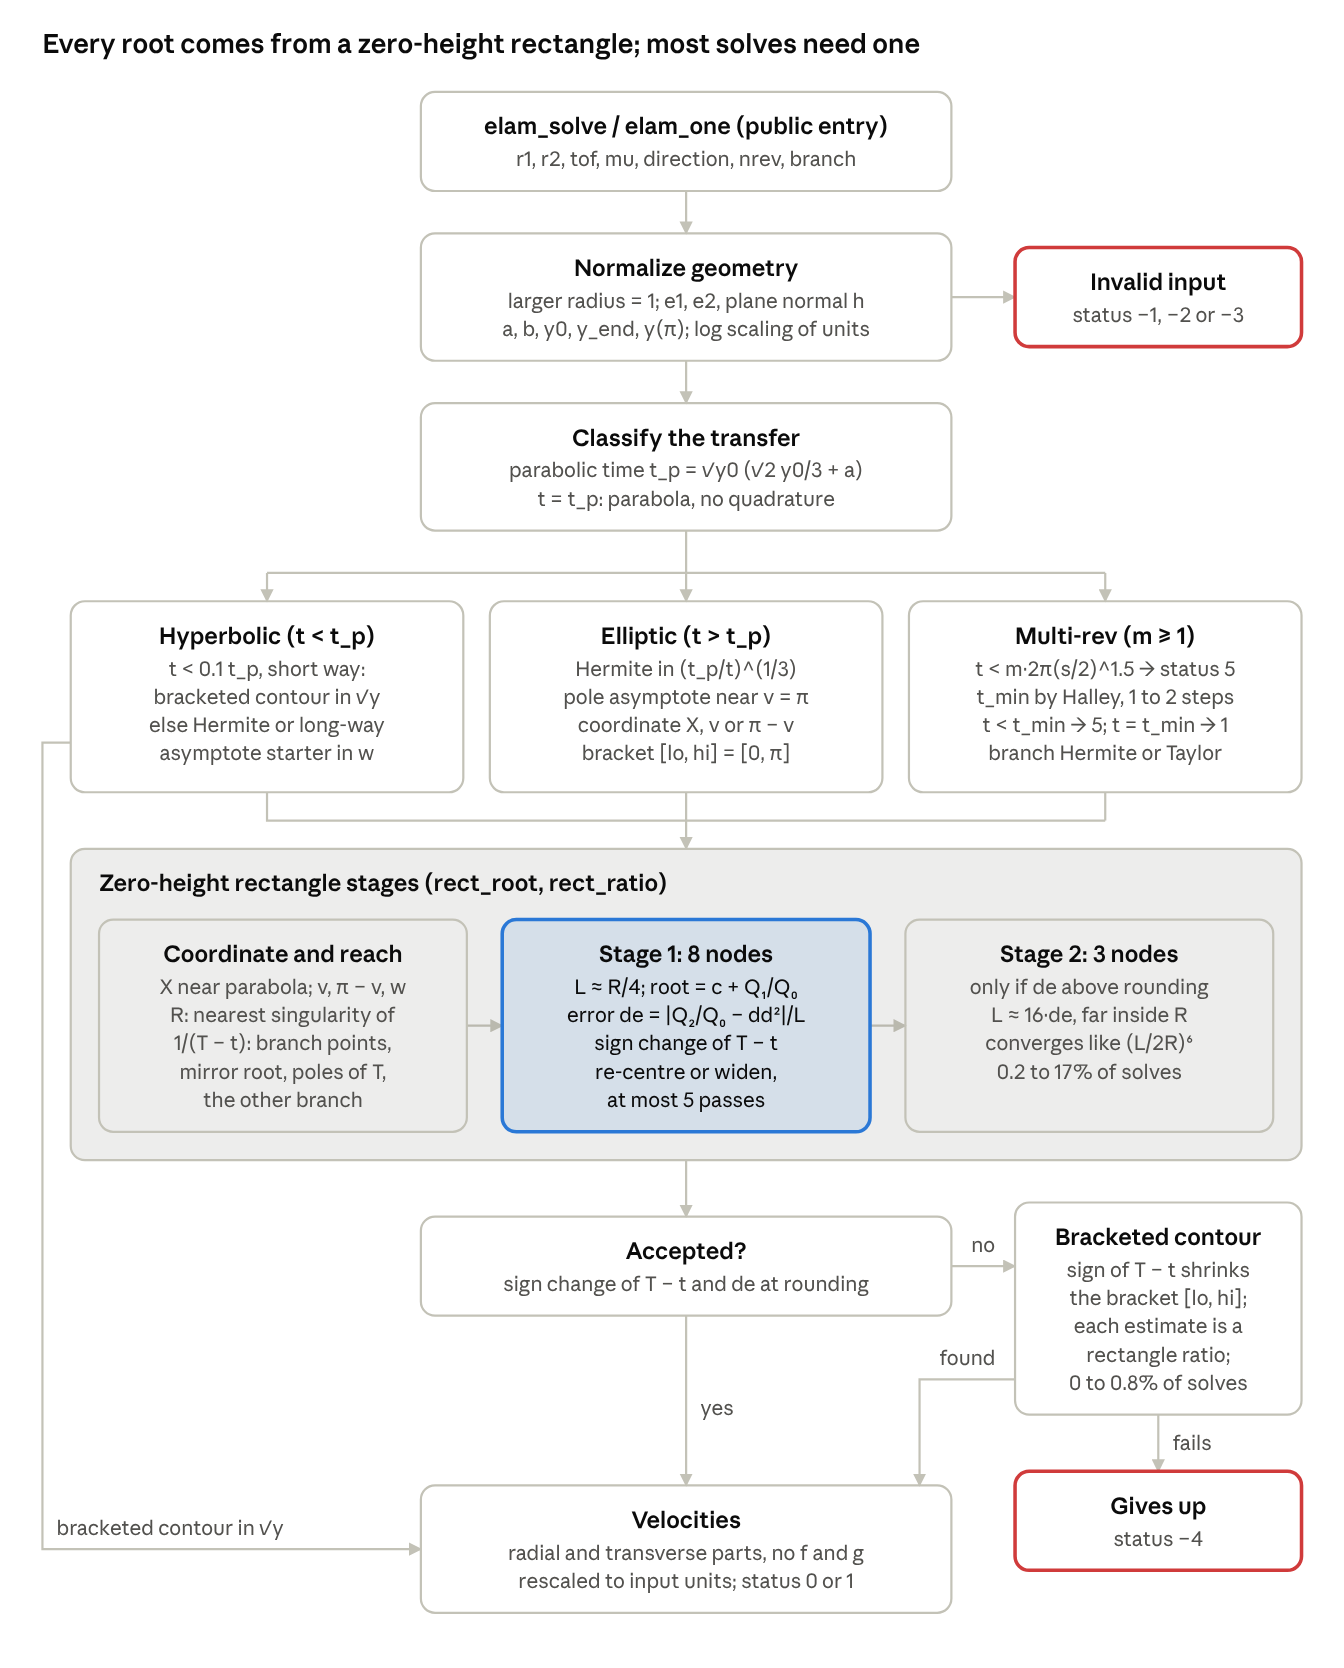
\includegraphics[width=\linewidth,height=0.85\textheight,keepaspectratio]{flowchart.png}
  \caption{EXCALI solve flow. The side branches are rare: stage 2 runs in 0.2 to 17\% of solves, depending on the class, and the bracketed contour in at most 0.8\%.}
\end{figure}

\begin{enumerate}
  \item \textbf{Normalize and check the geometry.} Divide by the larger radius, so it is exactly 1, and form unit vectors $e_1$, $e_2$ and the plane normal $h = e_1\times e_2$. Exactly antipodal endpoints need a supplied \code{plane\_normal}; coincident or same-ray endpoints return a status. Then form $|\cos(\theta/2)|$, $|\sin(\theta/2)|$, $a$, $b$, $y_0$, $y_\text{end}$ and $y(\pi)$. The dimensional \code{excali\_solve} scales through logarithms first, so inputs from $10^{-150}$ to $10^{150}$ work.
  \item \textbf{Classify and start (zero revolutions).} The parabolic time $t_p = \sqrt{y_0}\,(\sqrt2\,y_0/3 + a)$ decides the conic: $t>t_p$ is an ellipse, $t<t_p$ a hyperbola, and $t=t_p$ to rounding returns the parabola directly. A regime-specific closed-form starter gives $x$ and an admissible bracket $[\text{lo},\text{hi}]$.
  \item \textbf{Decide feasibility ($m>0$).} Reject $t < m\cdot2\pi\,(s/2)^{3/2}$ at once (status 5). Otherwise find the minimum time by Halley from the large-$m$ estimate, stopping as soon as feasibility is decided. Coalesced branches at the minimum return status 1. Each branch starter inverts a cubic Hermite in $\sqrt{1-(t_\text{min}/t)^{1/3}}$, or the local cubic Taylor model within 1\% of $t_\text{min}$.
  \item \textbf{Choose the coordinate.} Use $X=\pm x^2$ near the parabola, $v$ for an ellipse, $\pi-v$ near the upper pole, $w$ for a hyperbola, or $\sqrt{y}$ for the shortest hyperbolas.
  \item \textbf{Stage 1: 8-node zero-height rectangle.} Compute $R$ and set $L\approx R/4$, a power of two kept short of every pole of $T$. Evaluate $T$ and $T'$ at 8 Gauss--Legendre nodes and both endpoints in one fused loop, then form $d_d = \Q_1/\Q_0$, $d_e$ and the sign test. Accept when $|d_d|<0.8L$, $d_e<0.1L$ and $T-t$ changes sign. Otherwise re-centre on a consistent estimate, step toward it, or halve the growth factor, for at most 5 passes.
  \item \textbf{Stage 2: 3-node rectangle, only if needed.} If $d_e$ is above about $4\,\varepsilon_\text{mach}$ times the coordinate, run 3 nodes with $L\approx\min(R/16,\,16\,d_e)$ around the new centre. This happens in 0.2\% (fast hyperbolas) to 17\% (high eccentricity) of solves.
  \item \textbf{Bracketed contour, rarely.} If the stages fail, restore the state and keep taking zero-height rectangles inside a bracket that the sign of $T-t$ shrinks (0 to 0.8\% of solves).
  \item \textbf{Velocities.} Form radial and transverse components from the half-angle functions that the stages carried along, without Lagrange coefficients:
  \[
    v_{r1} = \delta_c - \frac{P}{\sqrt{r_1}}, \quad
    v_{r2} = -\Big(\delta_c + \frac{P}{\sqrt{r_2}}\Big), \quad
    v_{t1} = \sigma\frac{\sqrt{r_2}}{\sqrt{r_1}}, \quad
    v_{t2} = \sigma\frac{\sqrt{r_1}}{\sqrt{r_2}}.
  \]
  All four share the factor $\sqrt{2/y}$. $P$ comes from $\sqrt{r_1}-\sqrt{r_2}$, computed without cancellation, and $\delta_c$ is $\cos(\theta/2)$ minus the cosine of the anomaly, rearranged when the two are close. This avoids the cancellation that $f$ and $g$ suffer near $180^\circ$. The result is $v_1 = v_{r1}e_1 + v_{t1}(h\times e_1)$, and likewise for $v_2$.
\end{enumerate}

Status 0 means converged. The other codes are 1 (merged branches), 5 (below the minimum time), $-1$ (invalid input), $-2$ and $-3$ (degenerate geometry) and $-4$ (no convergence).

\section{Numerical engineering}

The method fixes the accuracy, and the remaining speed comes from removing library calls and divisions around it. None of these shortcuts touches the quadrature's accuracy: each one feeds only a starter or a distance estimate, or is exact to rounding.

{\small
\begin{tabularx}{\linewidth}{>{\raggedright\arraybackslash}p{3.6cm} >{\raggedright\arraybackslash}p{3.6cm} >{\raggedright\arraybackslash}X}
\toprule
Technique & Where it is used & Why \\
\midrule
Angle addition from compile-time tables & Node trigonometry in $v$ and $w$ & Tables hold cos/sin (cosh/sinh) of $L u/2$ for every $L=2^{-k}$, so each node costs a few multiplies and no trig call \\
\code{rotate} & Moving the centre between stages and into the velocities & Carries the centre's half-angle functions forward by a Taylor series of the shift, exact to rounding for shifts under 1/4 \\
\code{shch} & Every sinh/cosh pair & Taylor series for $|x|<0.5$, else one \code{exp}; replaced 7 library pairs and helps most on glibc \\
\code{rcbrt} & Starters & Cube root from the exponent bits plus one Halley step, $2\times10^{-5}$ relative; starters need only a few digits \\
\code{rlog}, \code{rasinh} & Branch-point distance $R$ & Fast logarithm to about $10^{-9}$; $R$ needs only its scale \\
\code{pow2m}, \code{kexp} & Power-of-two half-widths & From the bit pattern, avoiding gfortran's \code{\_\_powidf2} and \code{frexp} calls \\
One fused loop, two partial sums & \code{rect\_ratio} & Shortens the dependency chain: an 8-node stage costs about 35\,ns in $v$ (66 before) \\
Parabolic series in $X$ & Near $z=0$ & Removes the mirror root and the $v-\sin v\cos v$ cancellation \\
Long-way hyperbolic rearrangement & $b<0$, $w\ge0.3$ & Cancels large asymptotic terms algebraically \\
\bottomrule
\end{tabularx}
}

\paragraph{Portability.} The solver is standard Fortran 2008 plus C99 \code{cbrt} and \code{log1p}. The bit-pattern helpers assume IEEE-754 binary64, and a compile-time \code{ieee64} check switches them to standard intrinsics on any other format. CI builds and tests it on Linux x86-64, Linux ARM64 and macOS, with OpenMP on and off. There are no platform-specific paths.

\paragraph{Measured and not adopted.}
\begin{itemize}
  \item \textbf{Single-precision stage 1:} it then forces a double-precision stage 2 on every solve instead of about 10\%, a net loss.
  \item \textbf{Derivative-based (Tur\'an) quadrature using $T''$:} it would save under 6\,ns before its extra work.
  \item \textbf{Inline polynomial sin/cos:} no faster than the library pair. Apple's \code{\_\_sincos\_stret} gained 1\% and was rejected as nonportable.
  \item \textbf{Lockstep batching across problems:} not attempted. On two-double vectors the cost is a dependency chain within each solve.
\end{itemize}
A profile-guided build (\code{-DEXCALI\_PGO}) adds 3 to 5\%. It is optional and not used in the comparison.

\section{Accuracy and speed}

\paragraph{With the tables (2026-10-27).} Same benchmark, Apple M1 Pro, under background load (ratios reliable, absolute times to about $\pm5\%$). Single solves took 0.47 to 0.83 times ivLam's time (0.74 overall; ConfluentContour 0.92) before the double-double velocities and the single code path; now 0.88 overall (see \code{docs/VALIDATION.md}). By class: circular 0.75, elliptic short 0.77, elliptic long 0.82, high eccentricity 0.80, hyperbolic 0.83, near parabolic 0.76, multiple revolutions 0.65 to 0.70, infeasible 0.47, fast hyperbolas 0.78. On the classes it solves, Exact v2.2's serial kernel takes 213 to 227\,ns per call against EXCALI's 150 to 153. The batch entry takes 90 to 137\,ns per case, 101 overall. On the comparison's 1,000,000-case elliptic dataset, \code{excali\_batch} takes 118\,ns per case against 120 for Exact v2.2's vector batch and 133 for its serial batch. Errors at the 99th and 99.9th percentiles match or beat ConfluentContour's in every class and beat ivLam's except in the near-parabolic and fast-hyperbola classes; \code{docs/VALIDATION.md} has the tables. The rest of this section is the 2026-10-23 state before the tables.

EXCALI's maximum error is below ivLam's in 8 of the 10 feasible classes, by up to 160 times (high eccentricity). The other two are at rounding level for both solvers. Its speed relative to ivLam depends on the platform. The benchmark is \code{benchmark\_mixed}: 2,000 cases per class against quad-precision Kepler truth, one thread, \code{-O3 -fno-fast-math}, and zero failures for every solver. Errors are maximum relative endpoint-velocity errors on Apple silicon.

\begin{center}
\small
\begin{tabular}{l r r r r}
\toprule
& \multicolumn{2}{c}{EXCALI / ivLam time} & \multicolumn{2}{c}{Max error} \\
\cmidrule(lr){2-3}\cmidrule(lr){4-5}
Class & Apple M1 Pro & Linux x86-64 & ivLam & EXCALI \\
\midrule
circular\_short  & 0.80 & 1.09 & 3.6e-15 & 2.2e-15 \\
elliptic\_short  & 0.83 & 1.22 & 1.1e-13 & 4.4e-14 \\
elliptic\_long   & 0.91 & 1.16 & 3.4e-13 & 2.7e-14 \\
high\_ecc        & 1.00 & 1.34 & 1.6e-12 & 1.0e-14 \\
hyperbolic       & 0.90 & 1.40 & 2.2e-14 & 6.4e-15 \\
hyperbolic\_fast & 0.76 & 1.07 & 2.9e-15 & 6.8e-15 \\
near\_parabolic  & 0.90 & 1.39 & 1.5e-15 & 2.0e-15 \\
multirev\_1      & 1.10 & 1.31 & 8.4e-13 & 5.8e-13 \\
multirev\_2\_3   & 0.98 & 1.19 & 4.9e-13 & 2.2e-13 \\
multirev\_long   & 0.97 & 1.18 & 1.1e-12 & 3.9e-13 \\
infeasible\_m    & 0.40 & 0.61 & --- & --- \\
\midrule
\textbf{overall} & \textbf{0.91} & \textbf{1.18} & & \\
\bottomrule
\end{tabular}
\end{center}

The x86-64 column is from a GitHub Actions runner with GNU Fortran 13.3. Its per-class values predate the last \code{shch} change, which moved hyperbolic from 1.41 to 1.31 and the overall ratio from 1.21 to 1.18. The gap comes from glibc's slower sinh, cosh, cbrt and asinh, and from plain \code{-O3} on x86-64 not using fused multiply-add.

\paragraph{Other checks.}
\begin{itemize}
  \item \textbf{1,000,000-case elliptic dataset, 95,748 selected cases} (random, near $0^\circ/360^\circ$, near $180^\circ$): group maxima of $3.1\times10^{-13}$, $1.6\times10^{-14}$, $1.2\times10^{-12}$ and $6.9\times10^{-11}$. Near $180^\circ$ all solvers share the input-conditioning floor.
  \item \textbf{Multiple revolutions:} 32,400 feasibility decisions for 1 to 200 revolutions, from $10^{-1}$ down to $10^{-6}$ relative distance from the minimum time. All were classified correctly.
  \item \textbf{Edge cases:} independent propagation checks near antipodal and near coincident geometry, down to gaps of about $10^{-12}$\,rad, and unit scales from $10^{-150}$ to $10^{150}$.
  \item \textbf{MATLAB hard fixture:} 3,004 of 3,009, the same count and failing cases as ConfluentContour; Russell passes 3,003.
\end{itemize}
For scale along the version chain, the Exact documentation reports 918\,ns per problem for Exact v1 and 98.8\,ns for Exact v2.2. Those figures are on its own 5-million-case elliptic dataset, not this benchmark.

\paragraph{Where the time goes.} These are approximate phase costs for one solve on the M1 Pro, measured with builds that stop after each phase.
\begin{center}
\small
\begin{tabular}{l r r}
\toprule
Phase & Zero revolutions & Multiple revolutions \\
\midrule
Geometry & 23 ns & 23 ns \\
Starter & 12--35 ns & 110--135 ns \\
Stage setup (branch points, $R$, centre trig) & $\sim$20 ns & $\sim$20 ns \\
8-node rectangle kernel & $\sim$43 ns & $\sim$43 ns \\
Acceptance logic and the occasional stage 2 & $\sim$33 ns & $\sim$33 ns \\
Velocities & $\sim$19 ns & $\sim$19 ns \\
\midrule
\textbf{Total} & \textbf{165--205 ns} & \textbf{245--285 ns} \\
\bottomrule
\end{tabular}
\end{center}
The multi-revolution starter's minimum-time search was the largest single cost, and it is why ConfluentContour, which takes that minimum from a table, was faster on those classes until Step~10 did the same.

\section{Code breakdown}

\code{src/excali\_solver.f90} is 1,721 lines, 1,384 of them code, and includes the generated tables \code{src/excali\_tables.inc}. Every step exists once: \code{excali\_one} is \code{solve\_chunk} with one case, so single solves and the batch entry share all code. Lamberts-Comparison checks this repository out as \code{solvers/excali}, where EXCALI is solver ID 1 and the two Exact v2.2 originals are IDs 2 and 3.

{\small
\begin{tabularx}{\linewidth}{r r >{\raggedright\arraybackslash}p{3.7cm} >{\raggedright\arraybackslash}X}
\toprule
Lines & Code & Part & What it does \\
\midrule
1--82 & 51 & Module header & Constants, Gauss--Legendre nodes and weights, trig tables for every $L=2^{-k}$, series coefficients, the starter tables and the \code{frame} type \\
83--128 & 38 & \code{excali\_solve}, \code{excali\_one} & Dimensional entry (units through logarithms); one case through \code{solve\_chunk} \\
129--234 & 73 & \code{general\_root} & Table-free path: closed-form starters, multi-revolution feasibility bound \\
235--729 & 386 & Its contained procedures & Halley minimum time, stage 1 and 2 control, coordinate choice, singularity distance $R$, bracketed contours in $\sqrt{y}$ and in the anomaly \\
730--849 & 93 & \code{excali\_batch}, \code{solve\_chunk} & Blocks of up to 32 cases, stage by stage: geometry, tables, one rectangle, general path, velocities \\
850--1083 & 192 & Stage steps & \code{geometry}, \code{table\_coordinates}, \code{table\_root}, \code{fast\_coordinate}, \code{fast\_accept}, \code{velocities} (internal, inlined) \\
1084--1205 & 111 & \code{rect\_ratio} & The zero-height rectangle: fused node loop, $\Q_0$, $\Q_1$, $\Q_2$, $d_d$, $d_e$, sign test \\
1206--1332 & 116 & \code{rotate}, \code{f\_derivs}, \code{time\_derivs} & Half-angle functions by angle addition; $T$ and its derivatives in each coordinate \\
1333--1483 & 121 & Helpers & \code{shch}, \code{sincos\_half}, \code{pow2m}, \code{kexp}, \code{rasinh}, \code{qlog}, \code{rasin}, \code{rlog}, \code{rcbrt}, \code{xof} \\
1484--1618 & 117 & Table lookups & \code{table\_v}, \code{table\_w}, \code{near\_parabola\_x}, \code{mrev\_table} \\
1619--1722 & 86 & Velocity accuracy, helpers & \code{fhyp}, \code{fg\_velocities} (double-double Lagrange $f,g$), \code{lagrange4}, \code{hermite}, \code{cross} \\
\bottomrule
\end{tabularx}
}

The other files are \code{tools/gen\_tables.py} (the table generator), \code{src/exact\_adapter.f90} (wrappers for the preserved originals), \code{original/} (Exact v1 and v2.2, byte for byte), \code{tests/} (independent truth checks) and \code{docs/VALIDATION.md} (all measured results). The comparison repository adds \code{benchmark\_mixed}, the 50,000-case cross-solver test, the near-antipodal and near-coincident propagation tests and the MATLAB harness.

\end{document}
